\documentclass[12pt,technote]{IEEEtran}
\usepackage{cite}
\usepackage{amsmath}
\usepackage{hyperref}
\usepackage{bookmark}
\usepackage{amssymb}
\usepackage{graphicx}
\usepackage{caption}
\usepackage{subcaption}
\usepackage{hyperref}
\usepackage{tikz}

\usetikzlibrary{shapes.geometric, arrows}

\hypersetup{
    colorlinks=true,
    linkcolor=blue,
    filecolor=magenta,
    urlcolor=cyan,
    pdfpagemode=FullScreen,
}

\author{Henry Pick, MATH189J}
\title{Algebraic Signal Processing Theory in Image Processing}
\date{3 April 2022}
\begin{document}
\maketitle
\begin{abstract}
    In this paper, we explore constructs in image processing through the work of Markus P\"uschel on algebraic signal processing theory. His main objective was to introduce well-established concepts in signal processing in terms of a comprehensive algebraic theory. Here, we do much of the same, in fact a significant portion of this paper is devoted to reviewing essential ideas in his paper. We draw connections between abstract algebra and representation theory and the core concepts learned in many systems engineering classes. In my own effort to make this work original, I will explore several applied cases not covered in P\"uschel's work and design an image compression pipeline that makes use of several of P\"uschel's discussion points.
\end{abstract}
\section{Introduction}
In nearly all fields of the applied sciences, we interact with the broad definition of ``signal processing''. It is a term traditionally used in electrical engineering but has now found use in a wide range of other fields including image processing, wireless communication, financial analysis, and machine learning.

In the broadest sense, signal processing deals with functions defined on sets, often times countable sets in the context of digital computing. We also have a set of functions, commonly referred to as ``filters'' that transform these signals. In this paper, we focus on linear signal processing, which means that this set of functions operates on signals \textit{linearly}. That is, given a transformation $A$, signals $x$ and $y$, and scalar multiples $r_1$ and $r_2$ it holds that $A(r_1x + r_2y) = r_1A(x) + r_2A(y)$, which is still a signal.

To one with experience in one of the fields of signal processing, reading this last sentence should have been fairly straightforward, drawing on some assumptions. If one had contextualized this as the processing of complex digital sensor data, they might have assumed that $x$ and $y$ live in the vector space $\mathbb{C}^n$ over the field $\mathbb{C}$ and that the expression $r_1x + r_2y$ is simply the vector sum of $x$ and $y$ scaled by $r_1$ and $r_2$. Reading this last sentence from an abstract algebra perspective should have seemed slightly awkward, however. Since we have not given an algebraic foundation for these objects $A, x, y, r_1,$ and $r_2$, we have no conception of how the interact with one another, how we might represent these objects linearly, and what a signal generally represents. The instinct of the mathematician is to establish a comprehensive theory that characterizes features common to all signal processing contexts. This is exactly what Markus P\"uschel has done in his work on algebraic signal processing theory\cite{AlgebraicSignalProcessing2006}.

One might question the practical value of an algebraic exploration of already well-established science. In this inquiry, we find many justifications that apply far beyond the mathematics alone. For example, an engineer who has significant experience in one field of signal processing may find a natural means of recognizing parallels in an entirely different field. It also becomes clear that several tasks in processing research that are seemingly the product of ingenious creativity are actually quite procedural. The design of fast transform algorithms, for example, can be as simple as observing the symmetry structure of an underlying signal module.

The structure of this paper will first explore some of the foundational concepts introduced in the P\"uschel paper, which is primarily an expository section. In this section, we also consider some ideas that were not addressed in this work and potential extensions for P\"uschel's signal processing theory. We then move on to a practical application of constructing a signal model for images and a fast transform to be used in an image compression program.
\section{From First Principles}
In standard signal processing theory, signals live in a vector space like $\mathbb{C}^n$ over the base field, which gives the direct operations of signal addition and ``scalar multiplication''. This vector space structure also endows us with several other notions like dimension, basis, linear mappings and subspaces. We then encounter objects called filters, linear operators that act on signals to produce new signals. The operation of a filter on a signal is a different operation than the sum of two signals. We use the multiplication operation to represent this action of a filter on a signal
\begin{equation*}
    \text{filter}\cdot\text{signal} = \text{signal}
\end{equation*}
filtering also obeys the laws of distributivity
\begin{align*}
    &\text{filter}\cdot (\text{signal} + \text{signal}) \\
    =\ &\text{filter}\cdot \text{signal} + \text{filter}\cdot\text{signal}
\end{align*}
For $h,h'\in \mathcal{A}$ and $s,s'\in\mathcal{M}$ and $\alpha$ in the base field, we also have
\begin{align*}
    h\cdot (s + s') &= h\cdot s + h\cdot s'\\
    h\cdot (\alpha s) &= \alpha (h\cdot s)\\
    h'\cdot (h\cdot s) &= (h'\cdot h)\cdot s
\end{align*}
and filters can be operated on in various manners as well
\begin{align*}
    \text{filter} + \text{filter} &= \text{filter (parallel connection)}\\
    \text{filter} \cdot \text{filter} &= \text{filter (series connection)}\\
    \alpha\cdot\text{filter} &= \text{filter (amplification)}
\end{align*}
Beyond these properties, it must be mentioned that scalar multiplication of filters has left and right-distributivity and that multiplication by scalars is fully commutative with filter multiplication.
At this point, we see that the structure of this system can be defined using formal mathematical language. Our set of filters forms an algebra, which we refer to as $\mathcal{A}$. Our vector space is somehow operated on by $\mathcal{A}$, meaning it must have an associated $\mathcal{A}$-module called $\mathcal{M}$. However, it must be clearly stated that $\mathcal{M}$ does not necessarily equal $V$ as the operation of $\mathcal{A}$ on $\mathcal{M}$ is not strictly defined as an operation on a vector space. Thus, we must also define a bijection between $V$ and $\mathcal{M}$, which we call $\Phi$.

This is the central device in signal processing theory: a \textit{signal processing model} on a vector space $V$ consists of an ordered tuple $(\mathcal{A}, \mathcal{M}, \Phi)$ of algebraic objects as defined above. Through this model, we can exploit all of the mathematics of representation theory, harmonic analysis, and

One may note that as soon as $\Phi$ is defined, we have also given definitions for all of $V, \mathcal{M}$ and $\mathcal{A}$, meaning a signal model can be tersely expressed as this bijective function $\Phi$.

\subsection{Fourier Transforms}
Given that we have now associated the signal space with a module, we can define Fourier transforms on our signal space. For an arbitrary $\mathcal{A}$-module $\mathcal{M}$, let $M$ denote the set of all irreducible $\mathcal{A}$-submodules. In the general case, we cannot be certain that $\mathcal{M}$ can be decomposed into $M$ but in the case that
\begin{equation*}
    \mathcal{M} = \bigoplus_{\omega\in M}\omega
\end{equation*}
we have the machinery to construct a Fourier Transform for our signal model. Once we choose bases for the irreducible representations of $\mathcal{M}$ allows us to coordinatize this transformation, thus offering a linear representation which we will call $\mathcal{F}$.

\subsection{Shifts and the Z-Transform}

Anyone who has focused on control systems or electronics in engineering is likely familiar with the concept of transfer functions on signals and filters represented in the z-domain. For example, the z-transform as it pertains to signals over infinite continuous spaces is often the bilateral Laplace transform
\begin{equation*}
    X(s) = \mathcal{L}\{x(t)\} = \int_{-\infty}^\infty x(t)e^{-st}
\end{equation*}
as we note, one of the convenient properties of such a transform is that the multiplication of signals and filters in the z-domain is simple polynomial multiplication. This property is often given without any other context, but here we can trivially justify why this is the case.

\section{Space and Time Signals}

\section{Deriving Transforms from a Signal Model}

\cite{AlgebraicSignalProcessing2006}
Basic constructs in signal processing theory are filters, the z-transform, signals and the fourier transform. When we view them as they are classically taught, we see filters as linear operators and signals as a vector space, but this paper employs an algebraic perspective to show that these are more than

Z-transform converts a discrete time signal  into a complex frequency-domain representation, which can be thought of as the discrete time analogue of the Laplace transform. The

Define this notion of ``linear time invariance''


However, simple observation shows that this space is not closed under multiplication, the operation corresponding with successive filter application. As such, many engineering conventions treat this as multiplication of polynomials modulo $z^{-n}-1$

\subsection{Signal Shift Operator}
Every signal model that has the shift invariance property has a commutative filter algebra $\mathcal{A}$.
\section{Further Considerations: Transformations between Algebras}
Many times in engineering we encounter examples where a transformation may not transform to the same algebra and may not be invertible. For example, the process of downsampling a signal (commonly referred to as applying a decimating filter) applies a transformation that reduces the number of samples in a vector. This can be thought of as applying a filter with a large null space to a signal.

\section{Practical Example: Spectral Image Compression}
Data compression is a large subfield of information theory that involves the process of encoding information to use fewer bits than an original representation. Compressing data usually comes at the expense of additional computation, which is why the development of efficient compression algorithms is a central focus of this field. We focus specifically on lossy compression, in which information is lost through the compression processes (ie. the original data cannot be reconstructed from the compressed data) but the majority of useful information is preserved. One common lossy compression technique involves decomposing some signal into its irreducible representations and then discarding the less-meaningful representations. In this section we look at defining a signal model for digital image data and then develop a lossy compression technique based on an efficient transform derived from this signal model. There is also a source code accompaniment for this section which can be found \href{https://github.com/henry-2025/math189-spectral-compression}{here}.

\subsection{Choosing an Encoding}
There are a plethora of encodings for digital image data. Our goal here is to convert between two formats, one compressed and the other uncompressed. The uncompressed format is closest to the representation of raw sensor signal data while the compressed format is like one that we might wish to store on the hard drive of a computer. One family of encodings that stands out is the Netbpbm format, which encodes an image in a byte table corresponding directly to the pixel indices in the displayed image. For example, using the using red green and blue channel ordering for three-tuples, the following pixel array and color block are equivalent representations

\begin{center}
    $\begin{bmatrix}
        (255, 0, 0) & (0, 255, 0) & (0, 0, 255)\\
        (255, 255, 0) & (255, 255, 255) & (0, 0, 0)
    \end{bmatrix}$\\
    $\downarrow$\\
    
\includegraphics[width=0.5in]{figures/ppm_example.png}
\end{center}
As such, we will refer to our signal as a set of two-dimensional arrays of 8-bit unsigned integers for each color channel, which establishes our vector space $V$ for signals. We will say that elements in $V$ look like $\mathbf{s} = (s_{k,l})$, 2D arrays of elements in $s_{k,l}\in \mathbb{Z}/ 256\mathbb{Z}$. It may not make practical sense to think of this as a vector space right now, given that addition of signals and scalar multiplication seem like unnecessary operations. However, we hold this definition for the following section in which we derive the surrounding signal model.
\subsection{Signal Model}
In the discussion of shift operators, we found that spatial shifts are a necessary characteristic of data that does not have implicit directionality. We observed that for one dimensional signals, there exists only one shift operator that propagates outward from a single point in space. Here, we might intuitively think that one shift operator is also sufficient by just assigning the operator
\begin{equation*}
    q \diamond s_{x,y} = \frac{1}{4}(s_{x-1,y} + s_{x+1,y} + s_{x,y-1} + s_{x,y+1})
\end{equation*}
However, we soon realize see that this model would be flawed because we cannot reach all points in a 2d array from a single spatial operator. Instead, we define two spatial shifts, $q_x$ and $q_y$ and assign their propagations to each of the two dimensions such that
\begin{align*}
    q_x \diamond s_{x,y} &= \frac{1}{2}(s_{x-1,y} + s_{x+1,y})\\
    q_y \diamond s_{x,y} &= \frac{1}{2}(s_{x,y-1} + s_{x,y+1})
\end{align*}
Recalling the general module form for signal models with shift operators, we have defined $\mathcal{M}_x = \mathbb{C}[x]/p(x)$ to be a regular module with the basis $b_x = (p_0(x), \dots, p_{n-1}(x))$. If $x$ is the 1-dimensional shift operator for this signal model, we can naturally extend this to an $n$-dimensional analog with other shift operators $x_0, x_1, \dots, x_{n-1}$ in the module
\begin{equation}
    \mathcal{M}_{x_0, \dots, x_{n-1}} = \mathbb{C}[x_0, \dots, x_{n-1}]/\langle p(x_0), \dots, p(x_{n-1})\rangle
\end{equation}
Which has a basis that is the cartesian product of all bases of all the 1-dimensional submodules: $b_{x_0, \dots, x_{n-1}} = b_{x_0}\times \cdots \times x_{x_{n-1}}$. We shift our focus back to the 2-dimensional signal models pertaining to our processing of images. Suppose $x$ and $y$ are our spatial operators over the two axes and each has a dimension corresponding to the number of pixels in that axis, $k$ and $l$, respectively. Then we can extend the 1-dimensional signal model on the basis $(p_0, \dots, p_{n-1})$ to
\begin{equation*}
    \Phi(\mathbf{s}) = \sum_{0\leq k,l <n}s_{k,l}p_kp_l
\end{equation*}
We now take a detour into the formal definition of a tensor product of the two modules $\mathcal{M}_x$ and $\mathcal{M}_y$ and the associated algebra $\mathcal{A}_{x,y}$ thus has the same property:
\begin{align*}
    \mathcal{M}_{x,y} &= \mathcal{M}_x\otimes\mathcal{M}_y\\
    \mathcal{A}_{x,y} &= \mathcal{A}_x\otimes\mathcal{A}_y
\end{align*}
This observation gives a valuable insight for the construction of a fast fourier transform in this signal model. Because we are working with a signal whose
\begin{align*}
    \Delta : \mathbb{C}[x]&/p(x)\times\mathbb{C}[y]/p(y)\to\\
    &\bigoplus_{0\leq k,l<n}\mathbb{C}[x]/(x - \alpha_k)\times \mathbb{C}[y](y - \alpha_{l})
\end{align*}
This We already know that $\mathcal{M}_x$ and $\mathcal{M}_y$ are modules representing

The design of a fast 1D DCT goes beyond my understanding, but P\"uschel and other authors have published papers outlining algebraic approaches to its derivation\cite{puschel2003cooley,fastdct1988}. Instead, we will use one of many existing libraries with fast DCT-type 2 and DCT-type 3 algorithms. The trouble is that most operate exclusively on floating-point numbers which means that the available transforms are not written for our vector space in $(\mathbb{Z}/256\mathbb{Z})^{n^2}$. We address this by reinterpreting our vector space in $\mathbb{Q}^n$, performing all of our calculations as rational floating-point numbers, and then casting back down to the original vector space. Evidently, this is a cause for a large computation overhead and will almost certainly make our compression system slower than current state-of-the-art systems. The importance of matching a signal model to the data being processed is thus emphasized again, though I did not have time to address this issue in my project.

\subsection{Algorithm Design}
%TODO: explain the layout of the matrix in terms of frequency
Having designed a two-dimensional DCT that operates in $O(n^2\log{n})$ on floating-point $n\times n$ matrices, we shift our attention to designing a signal processing pipeline for image compression. There are two fundamental ideas behind most DCT-based image compression techniques: (1) at most resolutions, lower-frequency components occupy a bulk of the signal energy and perhaps consequentially, (2) higher-frequency components are less important to the characteristics of the image. Compression algorithms will find a means of stripping these high-frequency components out of the representation of their signal. Some encodings like JPEG do this in a nearly lossless manner by applying a normalization to these frequency components called quantization\cite{JPEG1992}. Quantization reduces all but the most powerful high-frequency components to zero leaving a frequency matrix that is very sparse in the lower-right region. The JPEG encoding employs a technique called ``zigzag scanning'' to encode these redundancies in a manner that will likely encode most of the zeros contiguously as shown in \ref{fig:zigzag}.
\begin{figure}[h]
    \begin{center}
        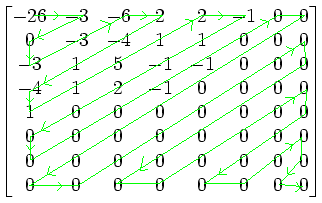
\includegraphics[width=2in]{figures/jpeg_zigzag.png}
    \end{center}
    \caption{The zigzag scanning used in JPEG intuitively maximizes the number of contiguous encountered in the frequency matrix}
    \label{fig:zigzag}
\end{figure}
In this compression scheme, we take a much simpler approach by simply taking the output matrix of the DCT type-2 and discarding the indices $k,l > m$ for $m \geq 1$ thereby constructing a low-rank approximation of the frequency matrix. This compression scheme is bound to have a higher data-loss rate as it simply ignores information that might be outside of this frame of the matrix. Relying on the assumption that most of the signal energy is concentrated in the lower spatial frequencies of the signal, this method should be a much better approximation than an arbitrary selection of $m\times m$ matrix elements.

One might be tempted to take this scheme and apply the transformation and rank reduction to the entire image in one two-dimensional DCT type-2. This method has two major flaws, the first being that our designed DCT only operates on square matrices while images can be any rectangular shape. We would have to either crop every image to a square or derive some type of padding scheme to extend the image bounds to a square. The second is that an unnecessary asymptotic complexity degree is used as our algorithm is $\mathcal{O}(n^2\log{n})$.

Instead, we can make our DCT a constant size and apply it to sub-matrices of the image. Our asymptotic runtime complexity is now $\mathcal{O}(n^2)$ and we have also somewhat solved the square image problem by reducing the proportions of the image that need to be padded or cropped. One question

The described process can be summarized in the following

\tikzstyle{startstop} = [rectangle, rounded corners, minimum width=2cm, minimum height=0.7cm,text centered, draw=black, fill=red!30]
\tikzstyle{filter} = [rectangle, minimum width=2cm, minimum height=0.7cm,text centered, draw=black, fill=green!50]
\tikzstyle{arrow} = [thick,->,>=stealth]


\begin{center}
    \begin{tikzpicture}[node distance=1cm]
        \node (image) [startstop, xshift=-2cm] {Image};
        \node (disassemble) [filter, right of=image, xshift=2cm] {Disassemble};
        \node (dct) [filter, below of=disassemble] {DCT II 2D};
        \node (reduce) [filter, left of=dct, xshift=-2cm] {Rank Reduce};
        \node (write) [startstop, below of=reduce, xshift=1cm] {Write Encoding};

        \node (read) [startstop, below of=write, yshift=-0.5cm] {Read Encoding};
        \node (augment) [filter, below of=read, xshift=-2cm] {Augment Matrices};
        \node (idct) [filter, right of=augment, xshift=2.5cm] {DCT III 2D};
        \node (reassemble) [filter, below of=idct] {Reassemble};
        \node (im) [startstop, left of=reassemble, xshift=-1.5cm] {Image};

        \draw [arrow] (image) -- (disassemble);
        \draw [arrow] (disassemble) -- (dct);
        \draw [arrow] (dct) -- (reduce);
        \draw [arrow] (reduce) -- (write);
        \draw [arrow] (read) -- (augment);
        \draw [arrow] (augment) -- (idct);
        \draw [arrow] (idct) -- (reassemble);
        \draw [arrow] (reassemble) -- (im);
    \end{tikzpicture}
\end{center}
I implemented this using fftw3 floating point dct transformations and a command-line program written in C. It achieves most of the functionality that I was hoping for with a few issues with rectangular dimensioned images. 
We first take an image and convert it into its uncompressed form, in this example, I have taken the following image and converted it into binary ppm:
\begin{figure}[h]
    \centering
    \begin{subfigure}[m]{0.3\textwidth}
        \centering
        
\includegraphics[width=\textwidth]{figures/lion_compressed.jpg}
        \caption{A high-resolution image with 75\% compression applied}
        \label{fig:lion}
    \end{subfigure}
    \hfill
    \begin{subfigure}[b]{0.3\textwidth}
        \centering
        
\includegraphics[width=\textwidth]{figures/b_compressed.jpg}
        \caption{A lower-resolution image with ``sharp'' features. Artifacts in the 75\% compression are more evident.}
        \label{fig:letter_b}
    \end{subfigure}
    \label{fig:compression_outputs}
    \caption{Two different outputs of the compression algorithm that demonstrate its performance.}
\end{figure}
\bibliographystyle{plain}
\bibliography{paper}
\end{document}